\documentclass[twoside]{book}

% Packages required by doxygen
\usepackage{fixltx2e}
\usepackage{calc}
\usepackage{doxygen}
\usepackage[export]{adjustbox} % also loads graphicx
\usepackage{graphicx}
\usepackage[utf8]{inputenc}
\usepackage{makeidx}
\usepackage{multicol}
\usepackage{multirow}
\PassOptionsToPackage{warn}{textcomp}
\usepackage{textcomp}
\usepackage[nointegrals]{wasysym}
\usepackage[table]{xcolor}

% Font selection
\usepackage[T1]{fontenc}
\usepackage[scaled=.90]{helvet}
\usepackage{courier}
\usepackage{amssymb}
\usepackage{sectsty}
\renewcommand{\familydefault}{\sfdefault}
\allsectionsfont{%
  \fontseries{bc}\selectfont%
  \color{darkgray}%
}
\renewcommand{\DoxyLabelFont}{%
  \fontseries{bc}\selectfont%
  \color{darkgray}%
}
\newcommand{\+}{\discretionary{\mbox{\scriptsize$\hookleftarrow$}}{}{}}

% Page & text layout
\usepackage{geometry}
\geometry{%
  a4paper,%
  top=2.5cm,%
  bottom=2.5cm,%
  left=2.5cm,%
  right=2.5cm%
}
\tolerance=750
\hfuzz=15pt
\hbadness=750
\setlength{\emergencystretch}{15pt}
\setlength{\parindent}{0cm}
\setlength{\parskip}{3ex plus 2ex minus 2ex}
\makeatletter
\renewcommand{\paragraph}{%
  \@startsection{paragraph}{4}{0ex}{-1.0ex}{1.0ex}{%
    \normalfont\normalsize\bfseries\SS@parafont%
  }%
}
\renewcommand{\subparagraph}{%
  \@startsection{subparagraph}{5}{0ex}{-1.0ex}{1.0ex}{%
    \normalfont\normalsize\bfseries\SS@subparafont%
  }%
}
\makeatother

% Headers & footers
\usepackage{fancyhdr}
\pagestyle{fancyplain}
\fancyhead[LE]{\fancyplain{}{\bfseries\thepage}}
\fancyhead[CE]{\fancyplain{}{}}
\fancyhead[RE]{\fancyplain{}{\bfseries\leftmark}}
\fancyhead[LO]{\fancyplain{}{\bfseries\rightmark}}
\fancyhead[CO]{\fancyplain{}{}}
\fancyhead[RO]{\fancyplain{}{\bfseries\thepage}}
\fancyfoot[LE]{\fancyplain{}{}}
\fancyfoot[CE]{\fancyplain{}{}}
\fancyfoot[RE]{\fancyplain{}{\bfseries\scriptsize Generated by Doxygen }}
\fancyfoot[LO]{\fancyplain{}{\bfseries\scriptsize Generated by Doxygen }}
\fancyfoot[CO]{\fancyplain{}{}}
\fancyfoot[RO]{\fancyplain{}{}}
\renewcommand{\footrulewidth}{0.4pt}
\renewcommand{\chaptermark}[1]{%
  \markboth{#1}{}%
}
\renewcommand{\sectionmark}[1]{%
  \markright{\thesection\ #1}%
}

% Indices & bibliography
\usepackage{natbib}
\usepackage[titles]{tocloft}
\setcounter{tocdepth}{3}
\setcounter{secnumdepth}{5}
\makeindex

% Hyperlinks (required, but should be loaded last)
\usepackage{ifpdf}
\ifpdf
  \usepackage[pdftex,pagebackref=true]{hyperref}
\else
  \usepackage[ps2pdf,pagebackref=true]{hyperref}
\fi
\hypersetup{%
  colorlinks=true,%
  linkcolor=blue,%
  citecolor=blue,%
  unicode%
}

% Custom commands
\newcommand{\clearemptydoublepage}{%
  \newpage{\pagestyle{empty}\cleardoublepage}%
}

\usepackage{caption}
\captionsetup{labelsep=space,justification=centering,font={bf},singlelinecheck=off,skip=4pt,position=top}

%===== C O N T E N T S =====

\begin{document}

% Titlepage & ToC
\hypersetup{pageanchor=false,
             bookmarksnumbered=true,
             pdfencoding=unicode
            }
\pagenumbering{alph}
\begin{titlepage}
\vspace*{7cm}
\begin{center}%
{\Large Telemetry \\[1ex]\large 1 }\\
\vspace*{1cm}
{\large Generated by Doxygen 1.8.13}\\
\end{center}
\end{titlepage}
\clearemptydoublepage
\pagenumbering{roman}
\tableofcontents
\clearemptydoublepage
\pagenumbering{arabic}
\hypersetup{pageanchor=true}

%--- Begin generated contents ---
\chapter{File Index}
\section{File List}
Here is a list of all documented files with brief descriptions\+:\begin{DoxyCompactList}
\item\contentsline{section}{/home/pi/telemetry/\hyperlink{logging_8hh}{logging.\+hh} \\*Logging for \hyperlink{telemetry_8cc}{telemetry.\+cc} }{\pageref{logging_8hh}}{}
\item\contentsline{section}{/home/pi/telemetry/\hyperlink{telemetry_8cc}{telemetry.\+cc} \\*The main file for running the telemetry system between the beehive, digesotr, weather station, and the M\+Q\+TT Broker }{\pageref{telemetry_8cc}}{}
\item\contentsline{section}{/home/pi/telemetry/\hyperlink{telemetry_8hh}{telemetry.\+hh} }{\pageref{telemetry_8hh}}{}
\end{DoxyCompactList}

\chapter{File Documentation}
\hypertarget{logging_8hh}{}\section{/home/pi/telemetry/logging.hh File Reference}
\label{logging_8hh}\index{/home/pi/telemetry/logging.\+hh@{/home/pi/telemetry/logging.\+hh}}


Logging for \hyperlink{telemetry_8cc}{telemetry.\+cc}.  


{\ttfamily \#include $<$spdlog/sinks/stdout\+\_\+sinks.\+h$>$}\newline
{\ttfamily \#include $<$spdlog/spdlog.\+h$>$}\newline
Include dependency graph for logging.\+hh\+:\nopagebreak
\begin{figure}[H]
\begin{center}
\leavevmode
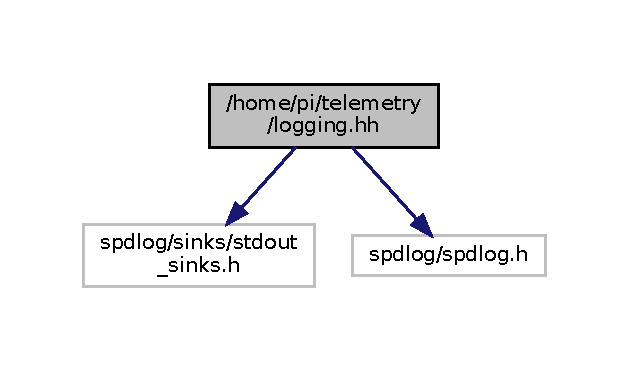
\includegraphics[width=302pt]{logging_8hh__incl}
\end{center}
\end{figure}
This graph shows which files directly or indirectly include this file\+:
\nopagebreak
\begin{figure}[H]
\begin{center}
\leavevmode
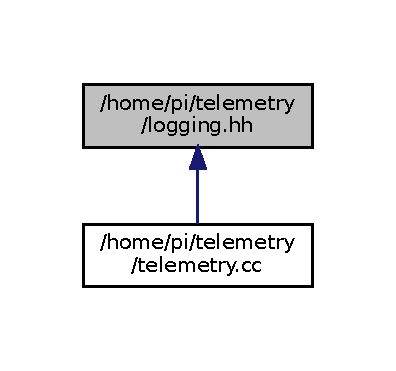
\includegraphics[width=190pt]{logging_8hh__dep__incl}
\end{center}
\end{figure}
\subsection*{Macros}
\begin{DoxyCompactItemize}
\item 
\mbox{\Hypertarget{logging_8hh_a3f987878202e572888e51b0010fe1dce}\label{logging_8hh_a3f987878202e572888e51b0010fe1dce}} 
\#define {\bfseries D\+E\+C\+L\+\_\+\+L\+O\+G\+G\+ER}(X)~extern decltype(spdlog\+::get(\char`\"{}\char`\"{})) X;
\item 
\mbox{\Hypertarget{logging_8hh_afe5ff6938e374f8ade78ba781a4a742e}\label{logging_8hh_afe5ff6938e374f8ade78ba781a4a742e}} 
\#define {\bfseries I\+N\+S\+T\+\_\+\+L\+O\+G\+G\+ER}(L\+O\+G\+G\+ER,  L\+O\+G\+G\+E\+R\+\_\+\+N\+A\+ME)~L\+O\+G\+G\+ER = std\+::make\+\_\+shared$<$spdlog\+::logger$>$(L\+O\+G\+G\+E\+R\+\_\+\+N\+A\+ME, console\+Sink);
\item 
\mbox{\Hypertarget{logging_8hh_a3e90f63040e6f216866895eec76c9792}\label{logging_8hh_a3e90f63040e6f216866895eec76c9792}} 
\#define {\bfseries D\+E\+F\+\_\+\+L\+O\+G\+G\+ER}(X)~decltype(spdlog\+::get(\char`\"{}\char`\"{})) X;
\end{DoxyCompactItemize}
\subsection*{Functions}
\begin{DoxyCompactItemize}
\item 
\hyperlink{logging_8hh_a25d3e12aaecd618c1176145894d5fb5a}{D\+E\+F\+\_\+\+L\+O\+G\+G\+ER} (mainlog)
\begin{DoxyCompactList}\small\item\em This is the defining of the various logs used within the program. If any more are to be added They need to be added here, in \hyperlink{logging_8hh}{logging.\+hh} and a little lower with the I\+N\+S\+T\+\_\+\+L\+O\+G\+G\+ER things later. \end{DoxyCompactList}\item 
\mbox{\Hypertarget{logging_8hh_a3458c74e904c52b76d3e427b4c195c50}\label{logging_8hh_a3458c74e904c52b76d3e427b4c195c50}} 
{\bfseries D\+E\+F\+\_\+\+L\+O\+G\+G\+ER} (networklog)
\item 
\mbox{\Hypertarget{logging_8hh_ab5cf5f3cabc1d43cc9485bc1906130a5}\label{logging_8hh_ab5cf5f3cabc1d43cc9485bc1906130a5}} 
{\bfseries D\+E\+F\+\_\+\+L\+O\+G\+G\+ER} (sensorslog)
\item 
\mbox{\Hypertarget{logging_8hh_a6cd81cbf58fc52813054048504855105}\label{logging_8hh_a6cd81cbf58fc52813054048504855105}} 
{\bfseries D\+E\+C\+L\+\_\+\+L\+O\+G\+G\+ER} (mainlog)
\item 
\mbox{\Hypertarget{logging_8hh_a954cb5a32e8c75d84ddb56b69dc4216f}\label{logging_8hh_a954cb5a32e8c75d84ddb56b69dc4216f}} 
{\bfseries D\+E\+C\+L\+\_\+\+L\+O\+G\+G\+ER} (networklog)
\item 
\mbox{\Hypertarget{logging_8hh_ad0daa0546f229bbbcde099a0a8630531}\label{logging_8hh_ad0daa0546f229bbbcde099a0a8630531}} 
{\bfseries D\+E\+C\+L\+\_\+\+L\+O\+G\+G\+ER} (sensorslog)
\end{DoxyCompactItemize}


\subsection{Detailed Description}
Logging for \hyperlink{telemetry_8cc}{telemetry.\+cc}. 

\begin{DoxyAuthor}{Author}
Daniel Ballif (\href{mailto:ballifdaniel@gmail.com}{\tt ballifdaniel@gmail.\+com}) 
\end{DoxyAuthor}


\subsection{Function Documentation}
\mbox{\Hypertarget{logging_8hh_a25d3e12aaecd618c1176145894d5fb5a}\label{logging_8hh_a25d3e12aaecd618c1176145894d5fb5a}} 
\index{logging.\+hh@{logging.\+hh}!D\+E\+F\+\_\+\+L\+O\+G\+G\+ER@{D\+E\+F\+\_\+\+L\+O\+G\+G\+ER}}
\index{D\+E\+F\+\_\+\+L\+O\+G\+G\+ER@{D\+E\+F\+\_\+\+L\+O\+G\+G\+ER}!logging.\+hh@{logging.\+hh}}
\subsubsection{\texorpdfstring{D\+E\+F\+\_\+\+L\+O\+G\+G\+E\+R()}{DEF\_LOGGER()}}
{\footnotesize\ttfamily D\+E\+F\+\_\+\+L\+O\+G\+G\+ER (\begin{DoxyParamCaption}\item[{mainlog}]{ }\end{DoxyParamCaption})}



This is the defining of the various logs used within the program. If any more are to be added They need to be added here, in \hyperlink{logging_8hh}{logging.\+hh} and a little lower with the I\+N\+S\+T\+\_\+\+L\+O\+G\+G\+ER things later. 


\begin{DoxyParams}{Parameters}
{\em main\+Log\+Level} & \\
\hline
\end{DoxyParams}

\hypertarget{telemetry_8cc}{}\section{/home/pi/telemetry/telemetry.cc File Reference}
\label{telemetry_8cc}\index{/home/pi/telemetry/telemetry.\+cc@{/home/pi/telemetry/telemetry.\+cc}}


The main file for running the telemetry system between the beehive, digesotr, weather station, and the M\+Q\+TT Broker.  


{\ttfamily \#include \char`\"{}telemetry.\+hh\char`\"{}}\newline
{\ttfamily \#include \char`\"{}logging.\+hh\char`\"{}}\newline
{\ttfamily \#include $<$iostream$>$}\newline
{\ttfamily \#include $<$getopt.\+h$>$}\newline
{\ttfamily \#include $<$confuse.\+h$>$}\newline
{\ttfamily \#include $<$vector$>$}\newline
Include dependency graph for telemetry.\+cc\+:
\nopagebreak
\begin{figure}[H]
\begin{center}
\leavevmode
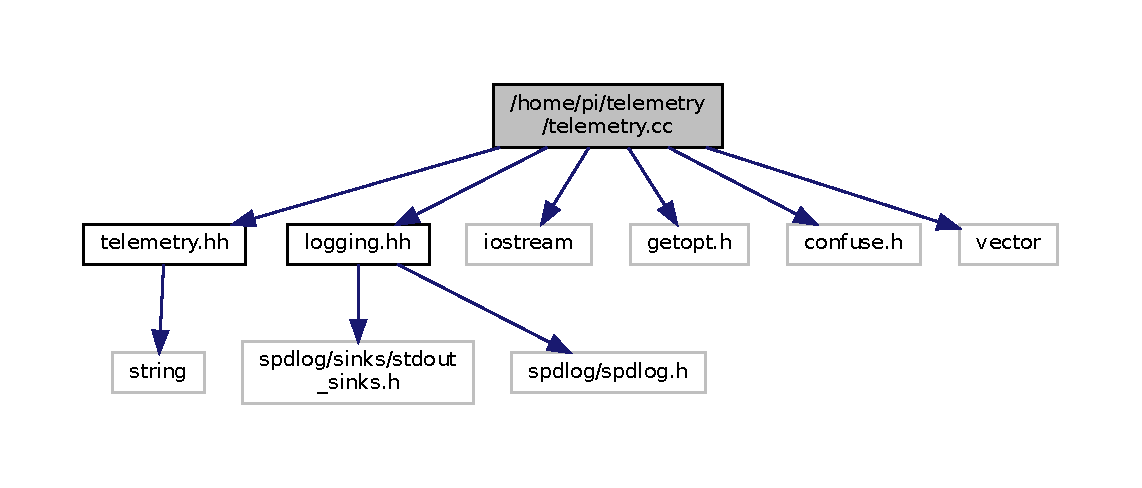
\includegraphics[width=350pt]{telemetry_8cc__incl}
\end{center}
\end{figure}
\subsection*{Functions}
\begin{DoxyCompactItemize}
\item 
int \hyperlink{telemetry_8cc_a0ddf1224851353fc92bfbff6f499fa97}{main} (int argc, char $\ast$argv\mbox{[}$\,$\mbox{]})
\end{DoxyCompactItemize}
\subsection*{Variables}
\begin{DoxyCompactItemize}
\item 
\mbox{\Hypertarget{telemetry_8cc_aab71f8b94719ede4dc9d04efb0ee8b19}\label{telemetry_8cc_aab71f8b94719ede4dc9d04efb0ee8b19}} 
cfg\+\_\+t $\ast$ \hyperlink{telemetry_8cc_aab71f8b94719ede4dc9d04efb0ee8b19}{cfg}
\begin{DoxyCompactList}\small\item\em declare the cfg variable to be used for configuration file. This is declared globably, so make sure not to declare it anywere else. \end{DoxyCompactList}\end{DoxyCompactItemize}


\subsection{Detailed Description}
The main file for running the telemetry system between the beehive, digesotr, weather station, and the M\+Q\+TT Broker. 

\begin{DoxyAuthor}{Author}
Daniel Ballif (\href{mailto:ballifdaniel@gmail.com}{\tt ballifdaniel@gmail.\+com}) 
\end{DoxyAuthor}


\subsection{Function Documentation}
\mbox{\Hypertarget{telemetry_8cc_a0ddf1224851353fc92bfbff6f499fa97}\label{telemetry_8cc_a0ddf1224851353fc92bfbff6f499fa97}} 
\index{telemetry.\+cc@{telemetry.\+cc}!main@{main}}
\index{main@{main}!telemetry.\+cc@{telemetry.\+cc}}
\subsubsection{\texorpdfstring{main()}{main()}}
{\footnotesize\ttfamily int main (\begin{DoxyParamCaption}\item[{int}]{argc,  }\item[{char $\ast$}]{argv\mbox{[}$\,$\mbox{]} }\end{DoxyParamCaption})}

This loop runs through the arguments given at the command line. The options are h (help), d (log), v (version), f (cfg\+File)

Setup a shared sink for all the different categories. Have to make that spdlog/sinks/stdout\+\_\+sinks.\+h. For setting up the logger see lines 305-\/308 of logging.\+cc in apsiproxy


\begin{DoxyParams}{Parameters}
{\em mainlog} & is instantiated. It will contain all of the logging for the main program. Most of the logging will occure here. \\
\hline
{\em sensorlog} & will contain all of the logging related to sensors, when they are registered, when they transfer data, etc. \\
\hline
{\em networklog} & will contain all of the network logging including M\+Q\+TT message logs.\\
\hline
\end{DoxyParams}
This is the section for setting up configuration paramaters. The first entry is the looked for file entry, the second is the default paramater, and the third is

Logging Setup in Cfg file. This allows for each of the following options. Default will be set to info.

cfg\+\_\+init must be called to initialize the parsing of the cfg file. if an error occurs, the cfg\+\_\+parse will throw and error and kill the program.

Libconfuse parsing. The first section will deal specifically with the logging options That have been setup in the configuration file. The second section will deal with the sensors section. For now, sensors will only be configurable in the file. However, logging needs to be configurable from the cmd line. cmd line will take precedence. If configured via cmd, 
\begin{DoxyParams}{Parameters}
{\em cmdlog} & will be set to 1. The sink will be console unless specified otherwise in cfg file.\\
\hline
\end{DoxyParams}
The next section run through the various cfg sections as created in the options section above. They are each added to a list. The index of each list correspond to one sensor. 
\begin{DoxyParams}{Parameters}
{\em sensors} & is the vector containing the names of each sensor, \\
\hline
{\em types} & is the vector containing the type of sensors used (ie. i2c, one-\/wire, etc). If these are not the same size the program will be killed.\\
\hline
\end{DoxyParams}

\hypertarget{telemetry_8hh}{}\section{/home/pi/telemetry/telemetry.hh File Reference}
\label{telemetry_8hh}\index{/home/pi/telemetry/telemetry.\+hh@{/home/pi/telemetry/telemetry.\+hh}}
{\ttfamily \#include $<$string$>$}\newline
Include dependency graph for telemetry.\+hh\+:\nopagebreak
\begin{figure}[H]
\begin{center}
\leavevmode
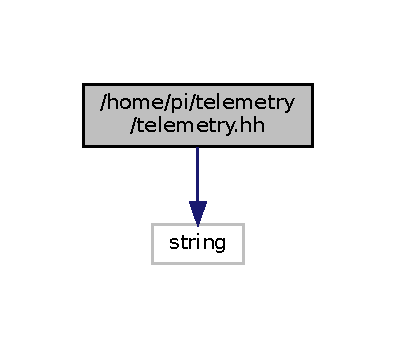
\includegraphics[width=190pt]{telemetry_8hh__incl}
\end{center}
\end{figure}
This graph shows which files directly or indirectly include this file\+:
\nopagebreak
\begin{figure}[H]
\begin{center}
\leavevmode
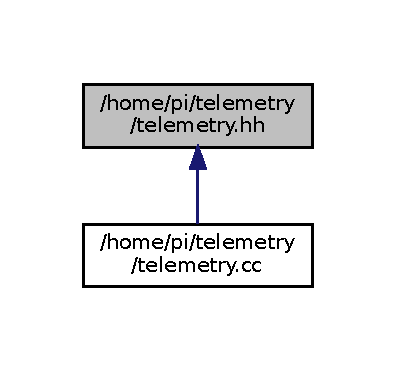
\includegraphics[width=190pt]{telemetry_8hh__dep__incl}
\end{center}
\end{figure}
\subsection*{Macros}
\begin{DoxyCompactItemize}
\item 
\mbox{\Hypertarget{telemetry_8hh_a3f45aded700251c1c65619ffef6bcd8f}\label{telemetry_8hh_a3f45aded700251c1c65619ffef6bcd8f}} 
\#define {\bfseries G\+E\+T\+O\+P\+T\+\_\+\+O\+P\+T\+S\+T\+R\+I\+N\+G\+\_\+\+P\+L\+A\+T\+F\+O\+RM}~\char`\"{}\char`\"{}
\item 
\mbox{\Hypertarget{telemetry_8hh_ae671aa30ca7aa44c6ca07a705d464974}\label{telemetry_8hh_ae671aa30ca7aa44c6ca07a705d464974}} 
\#define {\bfseries G\+E\+T\+O\+P\+T\+\_\+\+O\+P\+T\+S\+T\+R\+I\+N\+G\+\_\+\+C\+O\+M\+M\+ON}~\char`\"{}vhf\+:d\+:\char`\"{}
\item 
\mbox{\Hypertarget{telemetry_8hh_ae3217a88cef78a3de990b54a4e0d51e5}\label{telemetry_8hh_ae3217a88cef78a3de990b54a4e0d51e5}} 
\#define {\bfseries G\+E\+T\+O\+P\+T\+\_\+\+O\+P\+T\+S\+T\+R\+I\+NG}~G\+E\+T\+O\+P\+T\+\_\+\+O\+P\+T\+S\+T\+R\+I\+N\+G\+\_\+\+C\+O\+M\+M\+ON G\+E\+T\+O\+P\+T\+\_\+\+O\+P\+T\+S\+T\+R\+I\+N\+G\+\_\+\+P\+L\+A\+T\+F\+O\+RM
\end{DoxyCompactItemize}
\subsection*{Variables}
\begin{DoxyCompactItemize}
\item 
\mbox{\Hypertarget{telemetry_8hh_a728b969e374aba4020e39aea7e02e64f}\label{telemetry_8hh_a728b969e374aba4020e39aea7e02e64f}} 
std\+::string {\bfseries version} = \char`\"{}0.\+0.\+0\char`\"{}
\end{DoxyCompactItemize}


\subsection{Detailed Description}
\begin{DoxyAuthor}{Author}
Daniel Ballif (\href{mailto:ballifdaniel@gmail.com}{\tt ballifdaniel@gmail.\+com}) 
\end{DoxyAuthor}

%--- End generated contents ---

% Index
\backmatter
\newpage
\phantomsection
\clearemptydoublepage
\addcontentsline{toc}{chapter}{Index}
\printindex

\end{document}
